\documentclass[titlepage]{jsarticle}
\usepackage[dvipdfmx]{graphicx}
\usepackage{listings}
\usepackage{h31ec-exp}
\usepackage{biblatex}
\lstset{
  basicstyle={\ttfamily},
  identifierstyle={\small},
  commentstyle={\smallitshape},
  keywordstyle={\small\bfseries},
  ndkeywordstyle={\small},
  stringstyle={\small\ttfamily},
  frame={tb},
  breaklines=true,
  columns=[l]{fullflexible},
  numbers=left,
  xrightmargin=0zw,
  xleftmargin=3zw,
  numberstyle={\scriptsize},
  stepnumber=1,
  numbersep=1zw,
  lineskip=-0.5ex
}
\renewcommand{\lstlistingname}{ソースコード}
\makeatletter
\newcommand{\figcaption}[1]{\def\@captype{figure}\caption{#1}}
\newcommand{\tblcaption}[1]{\def\@captype{table}\caption{#1}}
\makeatother
\title{論理回路の設計}
\grade{3年32番}
\author{平田 蓮}
\team{第4班}
\date{2019年12月17日}
\expdate{2019年11月25日, 12月9日, 12月16日}
\coauthor{8番 小林歩夢}

\begin{document}
\maketitle
\section{目的}
  本実験では, ロジック学習装置KENTAC 2600 (昭和電業社) を用いて基本的な論理回路の設計を行い,
  コンピュータのハードウェア設計の基礎となる論理回路設計の理解を深めることを目的とする.
  まず, マルチプレクサや半加算器などの組み合わせ論理回路の設計に取り組み,
  真理値表と論理式と論理回路の対応へのイメージを深める.
  そして, 各種フリップフロップの動作確認とシフトレジスタ及びカウンタの設計を通して,
  コンピュータの記憶装置を用いた機能の基礎となる順序回路への理解を深める.
\section{KENTAC 2600について}
  本実験で使用するロジック学習装置KENTAC 2600の主な特徴を以下に挙げる.
  \begin{itemize}
    \item 入出力の端子とLEDディスプレイを接続することで, High/Lowを目で確認できる.
    \item 回路素子記号がパネル上に描かれているため, わかりやすい.
    \item 信号発信器を内蔵しているので, 外部の発信器が必要ない.
  \end{itemize}
\section{組み合わせ論理回路の設計}
  \subsection{プライオリティエンコーダの設計}
    情報を保存したり伝送したりする際には, なるべく使用する記憶素子や伝送路を少なくするのが望ましい.
    そこで用いられるのが符号化(エンコード)という手法であり, 符号化を行う回路をエンコーダという.
    中でも, 複数の入力があった場合に最も添字が大きい入力を優先させる回路を
    プライオリティエンコーダという.

    この節では, 4入力のプライオリティエンコーダを設計する.
    入力をそれぞれ$A_i$ ($i \in \{0, 1, 2, 3\}$), 出力を$Z_1, Z_2, E$とし,
    $(Z_2 \ Z_1)_2$で入力されている最大の添字を表す.
    $E$はどこからも1の入力がなければ1, それ以外の場合は0である.

    まず, このプライオリティエンコーダの真理値表を表\ref{tab:priority_encoder}示す.
    表内の$\times$はドントケア入力であることを示す.
    \begin{table}[h]
      \caption{4入力プライオリティエンコーダの真理値表}
      \label{tab:priority_encoder}
      \centering
      \begin{tabular}{cccc||ccc}
        \hline
        $A_0$ & $A_1$ & $A_2$ & $A_3$ & $Z_2$ & $Z_1$ & $E$ \\ \hline \hline
        0 & 0 & 0 & 0 & 0 & 0 & 1 \\
        1 & 0 & 0 & 0 & 0 & 0 & 0 \\
        $\times$ & 1 & 0 & 0 & 0 & 1 & 0 \\
        $\times$ & $\times$ & 1 & 0 & 1 & 0 & 0 \\
        $\times$ & $\times$ & $\times$ & 1 & 1 & 1 & 0 \\ \hline
      \end{tabular}
    \end{table}

    次に, この表からカルノー図を作成して各出力の式を導出する.
    カルノー図を以下に示す.
    \begin{center}
      \begin{figure}[h]
        \begin{minipage}{0.33\hsize}
          \centering
          \includegraphics[width=5cm]{images/Z2Karnaugh.pdf}
          \caption{$Z_2$についてのカルノー図}
        \end{minipage}
        \begin{minipage}{0.33\hsize}
          \centering
          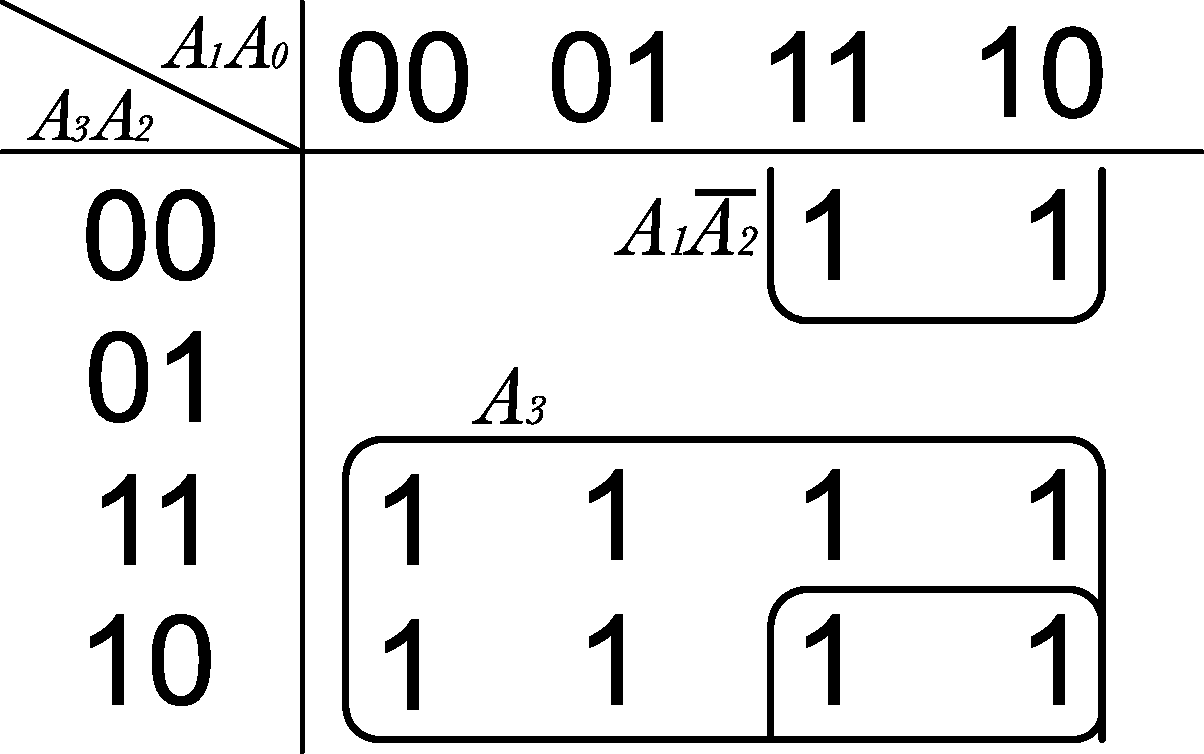
\includegraphics[width=5cm]{images/Z1karnaugh.pdf}
          \caption{$Z_1$についてのカルノー図}
        \end{minipage}
        \begin{minipage}{0.33\hsize}
          \centering
          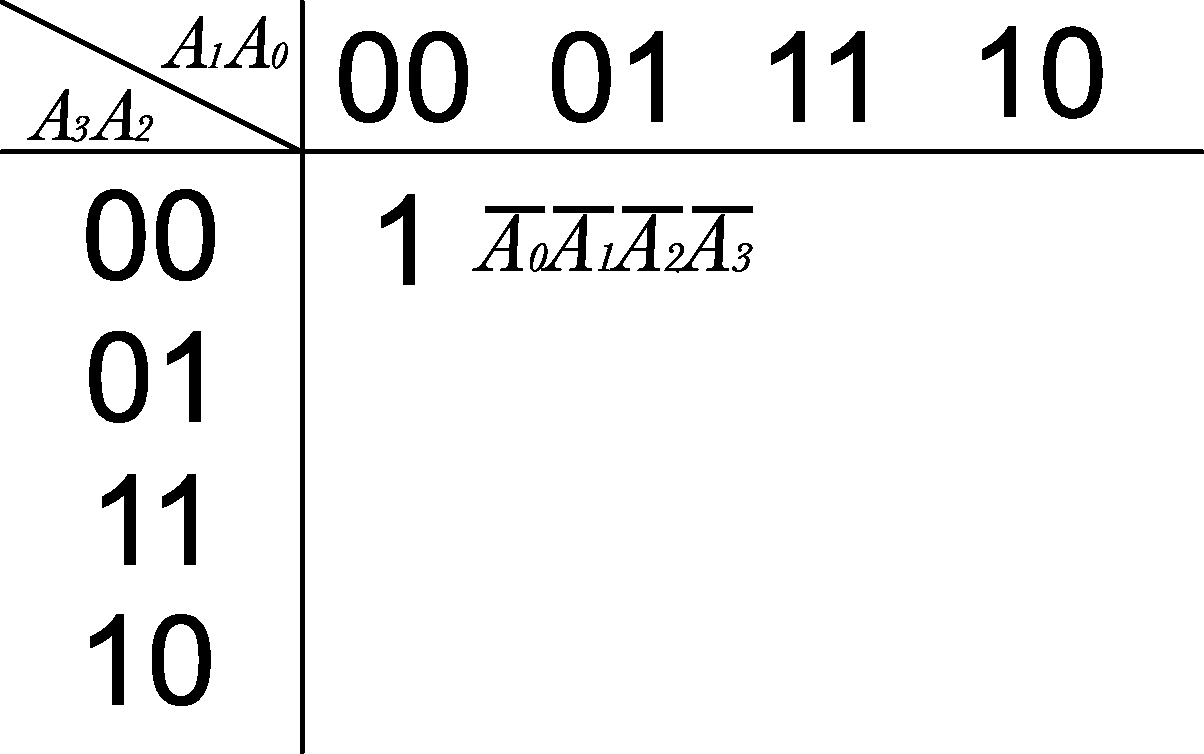
\includegraphics[width=5cm]{images/Ekarnaugh.pdf}
          \caption{$E$についてのカルノー図}
        \end{minipage}
      \end{figure}
    \end{center}

    また, これらの式は以下のように真理値表から直接求めることもできる.
    \begin{eqnarray*}
      Z_2 &=& A_2 \overline{A_3} + A_3 =
        A_2 \overline{A_3} + A_2A_3 + \overline{A_2}A_3 =
        A_2 + A_3 \\
      Z_1 &=& A_1 \overline{A_2} \ \overline{A_3} + A_3 =
        A_1 \overline{A_2} \ \overline{A_3} + A_1 \overline{A_2}A_3 +
          \overline{A_1 \overline{A_2}} A_3 =
        A_1 \overline{A_2} + A_3 \\
      E &=& \overline{A_0} \ \overline{A_1} \ \overline{A_2} \ \overline{A_3}
    \end{eqnarray*}
    最後に, これらの式から回路を構成する.
    構成した回路を図\ref{fig:priority_encoder}に示す.
    \begin{figure}[h]
      \centering
      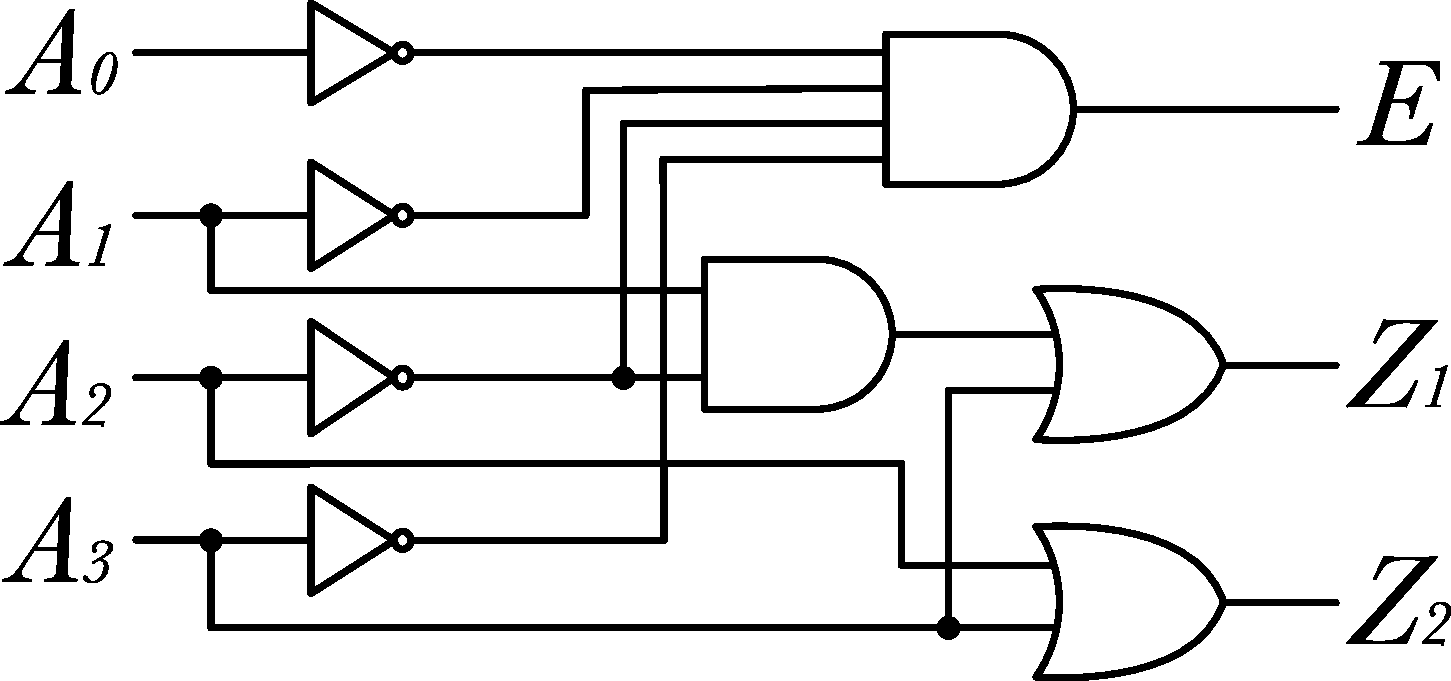
\includegraphics[width=10cm]{images/priority.pdf}
      \caption{4入力プライオリティエンコーダの論理回路}
      \label{fig:priority_encoder}
    \end{figure}
  \subsection{加算器} \label{subsec:FA}
    論理回路によって桁上がり入力を考慮しない1ビットの加算を行う回路を半加算器(HA: Half Adder)という.
    HAは, 入力$A$, $B$に対してその和$(C^+ \ S)_2$を出力する($C^+$は桁上がり).

    HAは下位ビットからの桁上がりを考慮していないので複数桁の演算をできないため,
    桁上がり入力$C$を追加することを考える.
    この回路を全加算器(FA: Full Adder)という.

    FAは, $A + B + C$を演算するので, HAを2つ使用して以下のように構成できる.
    ただし, 2つのHAの出力をそれぞれ$(C_1^+ \ S_1)_2$, $(C_2^+ \ S)_2$とする.
    \begin{enumerate}
      \item HAを使用して$A + B$を演算して$S_1$と$C_1^+$を得る.
      \item HAを使用して$S_1 + C$を演算して$S$と$C_2^+$を得る.
      \item 上のどちらかの演算で桁上がりが発生していたら全体の演算でも桁上がりが発生するので,
        $C_1^+$と$C_2^+$の論理和を取って$C^+$を得る.
    \end{enumerate}
    このように構成した回路とFAのタイミングチャートをを図\ref{fig:full_adder},
    \ref{fig:full_adder_timing}に示す.

    \begin{figure}[h]
      \begin{minipage}{0.495\hsize}
        \centering
        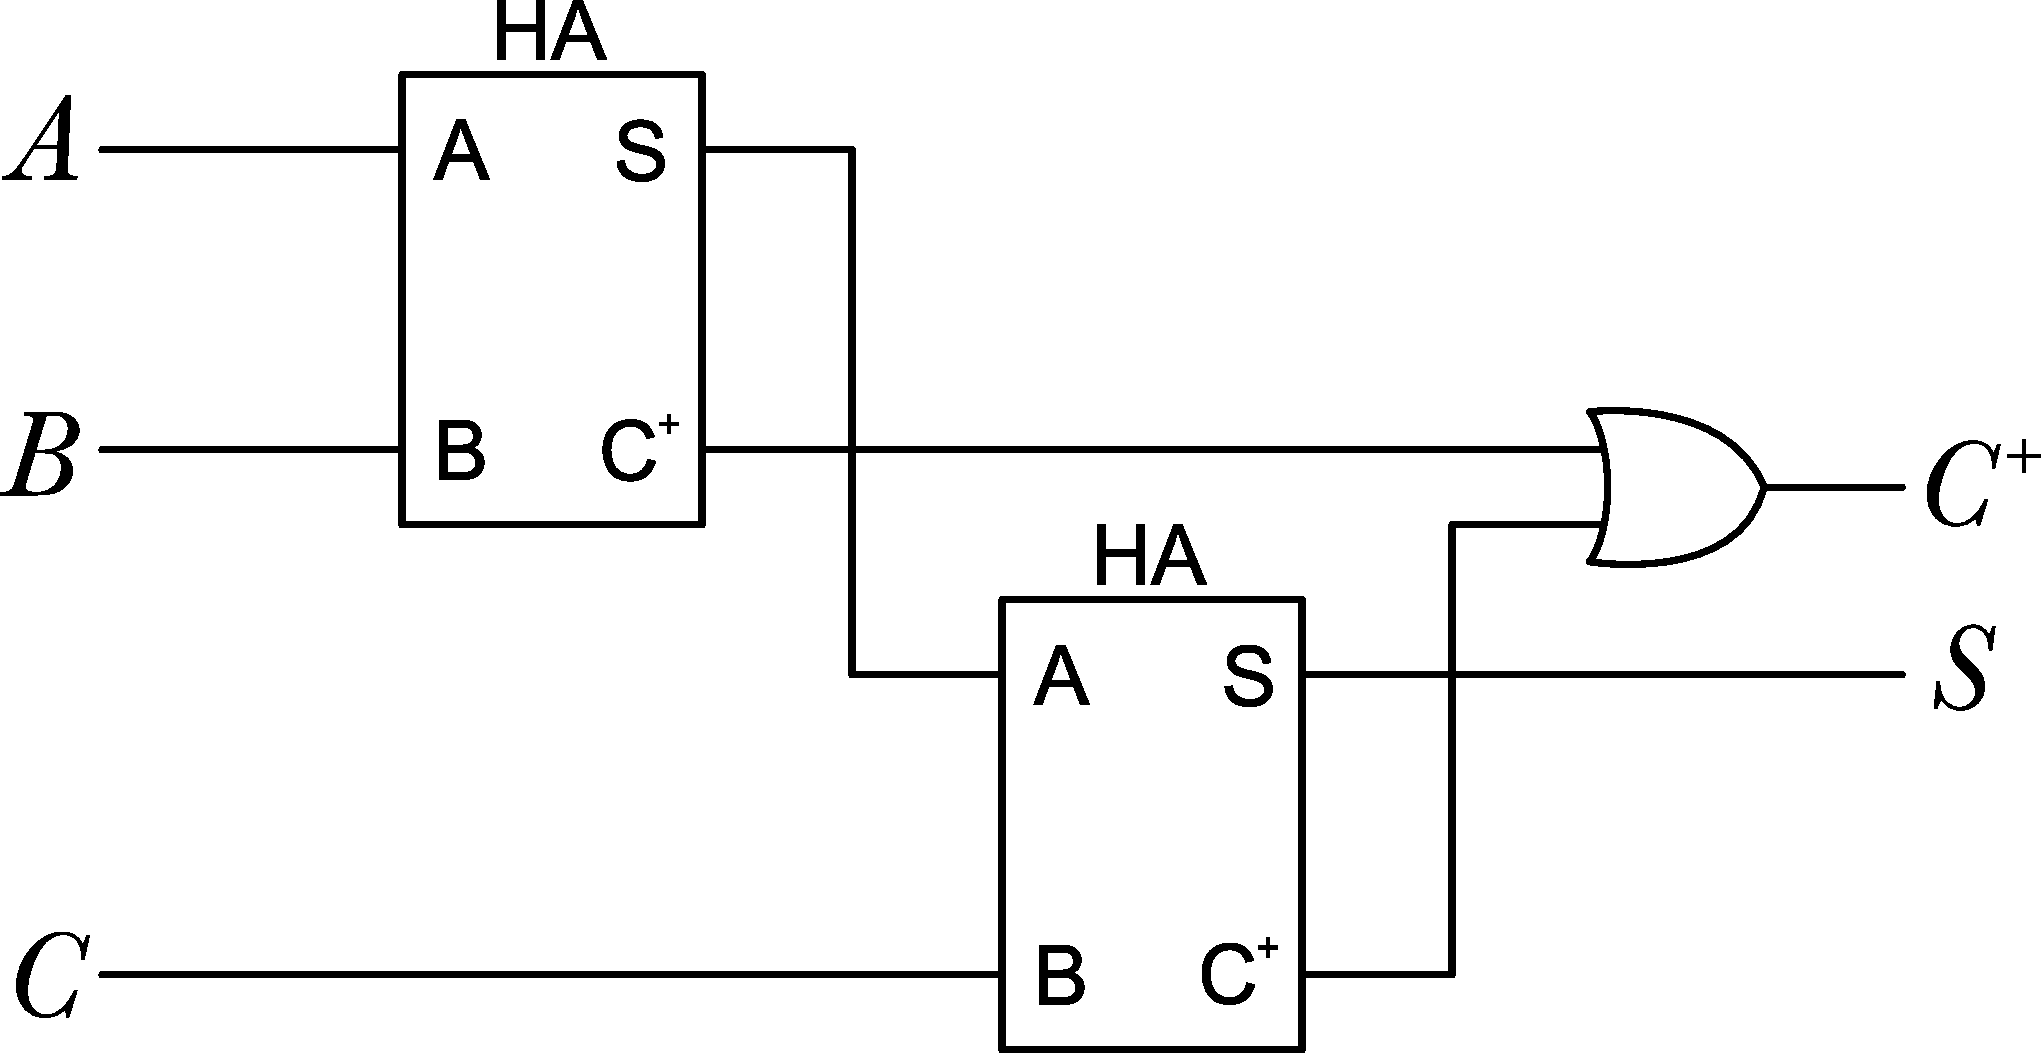
\includegraphics[width=7cm]{images/fa.pdf}
        \caption{FAの論理回路}
        \label{fig:full_adder}
      \end{minipage}
      \begin{minipage}{0.495\hsize}
        \centering
        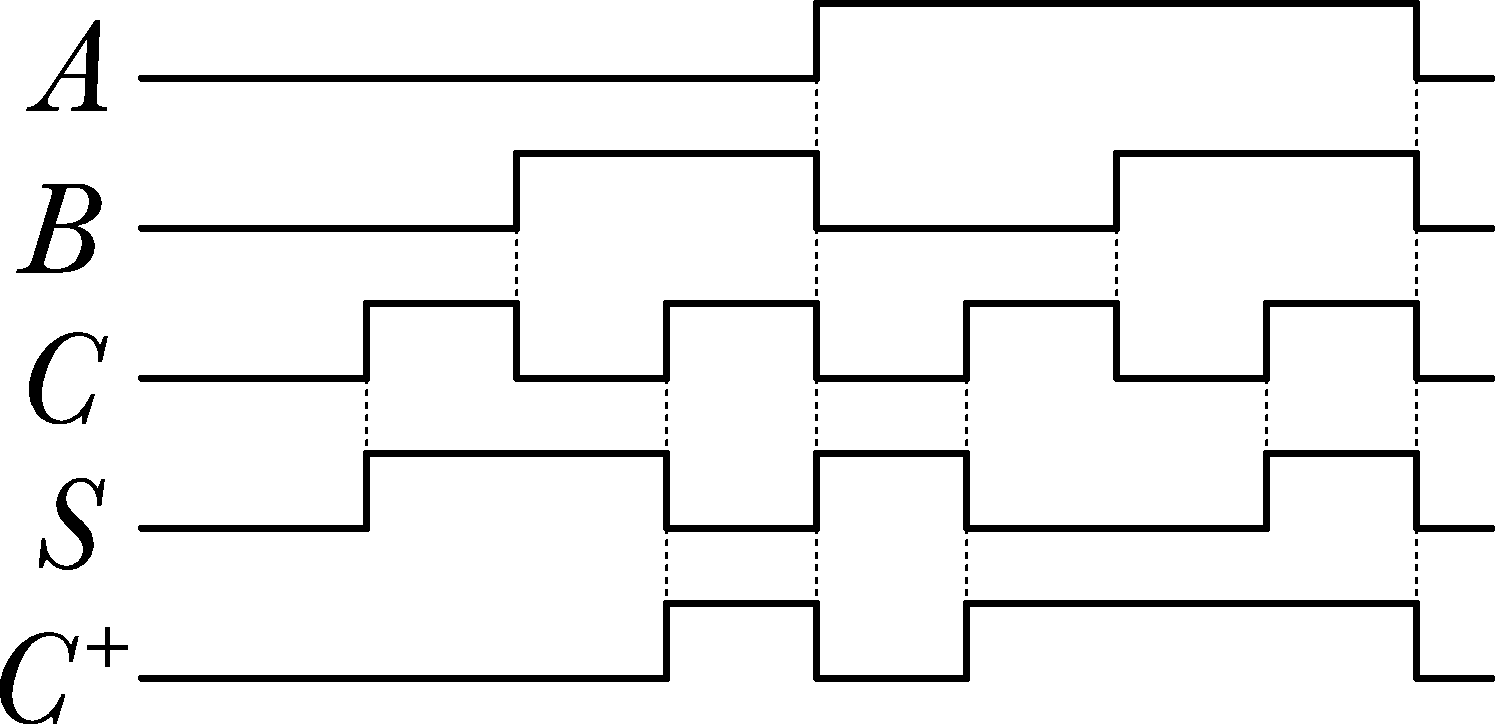
\includegraphics[width=7cm]{images/fa_timing.pdf}
        \caption{FAのタイミングチャート}
        \label{fig:full_adder_timing}
      \end{minipage}
    \end{figure}
  \subsection{2ビット加算器}
    \ref{subsec:FA}節で作成したFAを使用して, $(A_2 \ A_1)_2 + (B_2 \ B_1)_2 = (S_3 \ S_2 \ S_1)_2$
    の演算を行う2ビットの加算器を作成する.

    筆算と同じ要領で, 先に下位ビットをHAで演算した後, その桁上がりと上位ビットをFAで演算することで構成できる.
    図\ref{fig:2bit_adder}に作成した回路示す.
    \begin{figure}[h]
      \centering
      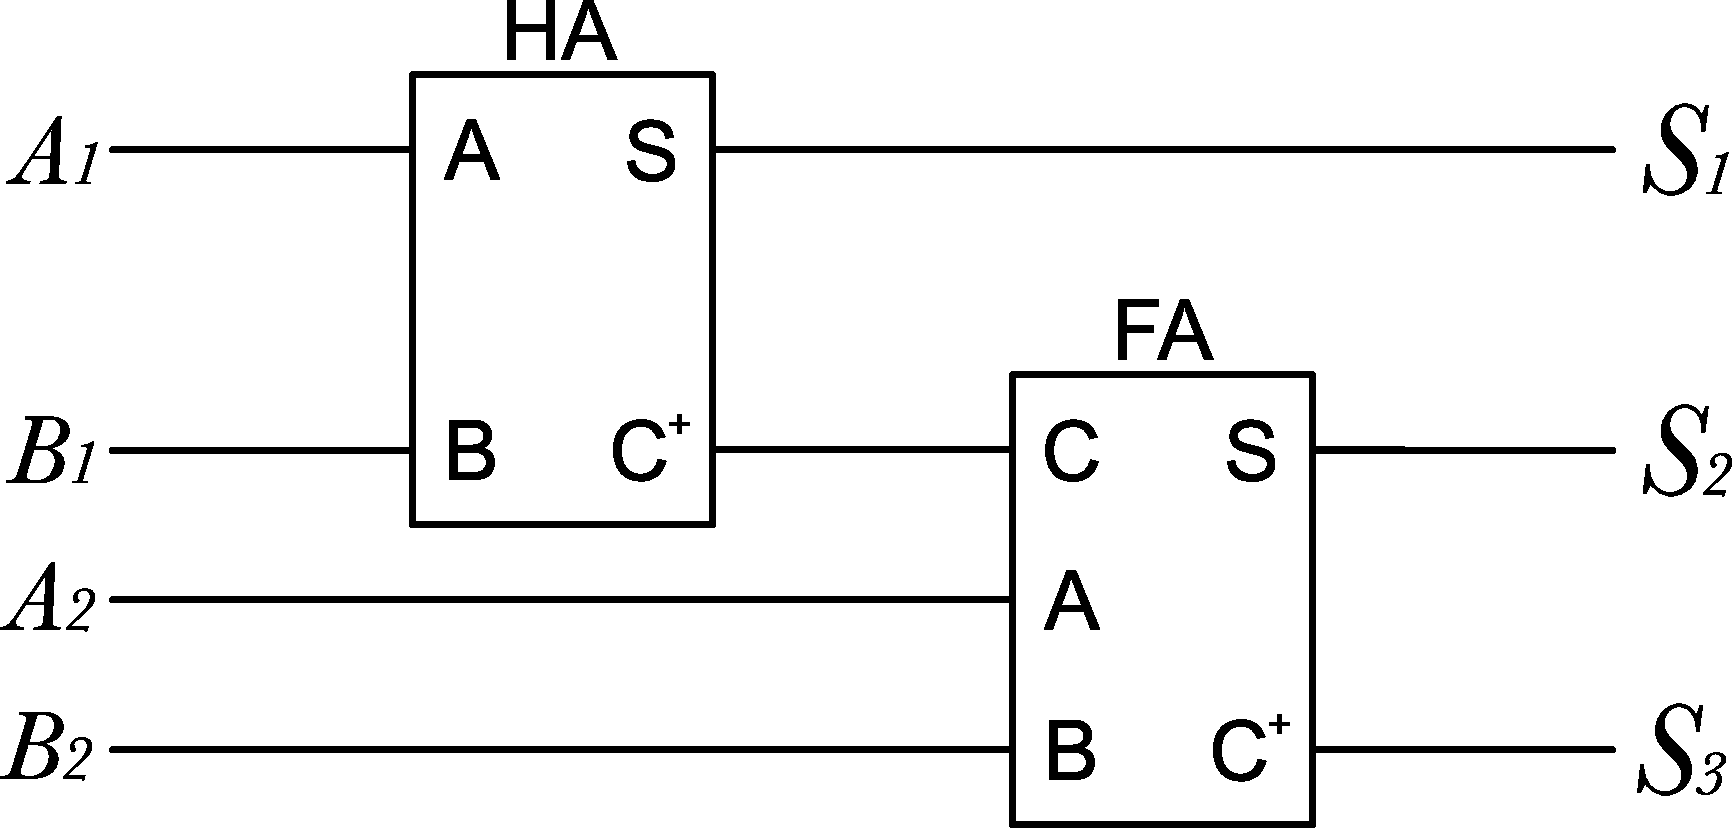
\includegraphics[width=10cm]{images/2bit.pdf}
      \caption{2ビット加算器の論理回路}
      \label{fig:2bit_adder}
    \end{figure}
\section{順序論理回路の設計}
  組み合わせ論理回路はその時の入力によって出力がただ1つに定まる回路であった.
  しかし, コンピュータの動作の中にはその時の入力だけでなく, その時の内部状態も出力に関わる物が多い.
  このような回路を順序回路という.
  順序回路はその時の入力と内部状態によって出力(次の内部状態状態)が決まるので,
  組み合わせ論理回路と違い, 入力に対して出力が一意に定まらない.

  順序回路を構成する際に, 1ビットの記憶素子としてフリップフロップ(FF: Flip Flop)を使用する.
  FFはその特徴によって様々な種類が存在するが, 本節ではJK-FFとD-FFに触れる.
  \subsection{JK-FFとD-FF} \label{subsec:jk_and_d}
    JK-FF, D-FFの入力をそれぞれ$(J, K), D$, 両FFのクロック入力,
    内部状態, 次の内部状態をそれぞれCLK, $Q$, $Q^+$とする.
    両FFのタイミングチャート, 状態遷移表を以下に示す.
    状態遷移表の$\times$はドントケア入力を表す.
    \begin{figure}[h]
      \begin{minipage}{0.495\hsize}
        \centering
        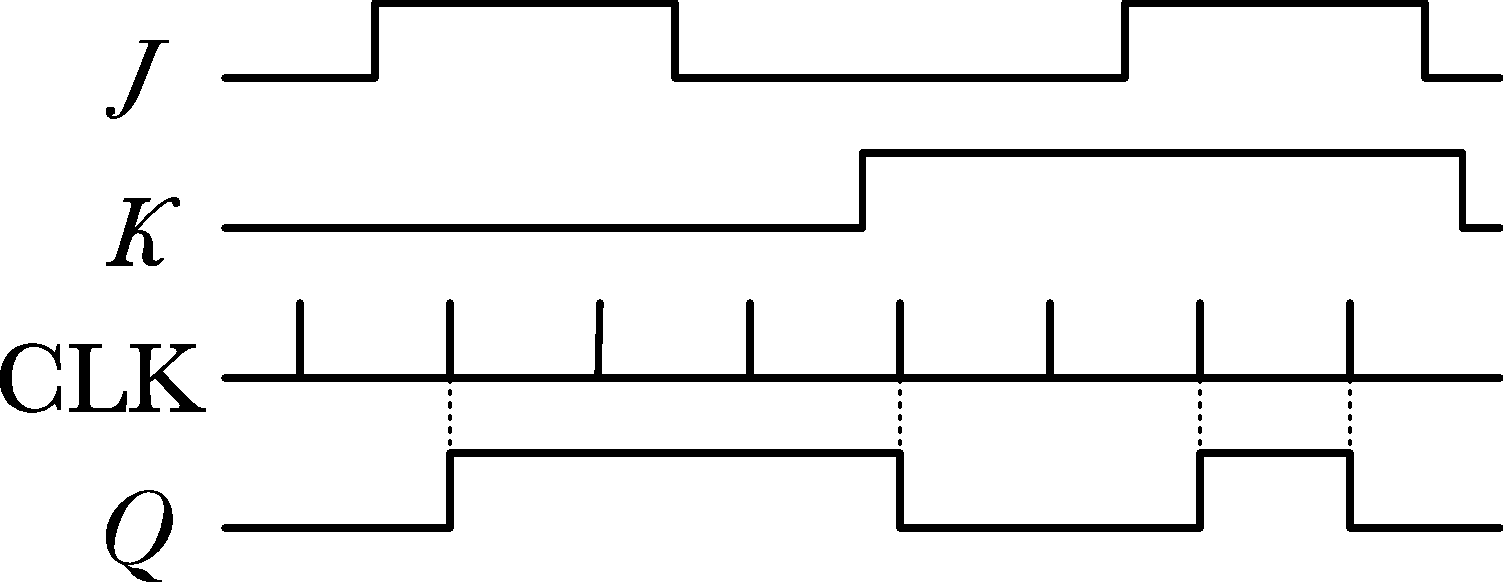
\includegraphics[width=7cm]{images/jk_timing.pdf}
        \caption{JK-FFのタイミングチャート}
      \end{minipage}
      \begin{minipage}{0.495\hsize}
        \centering
        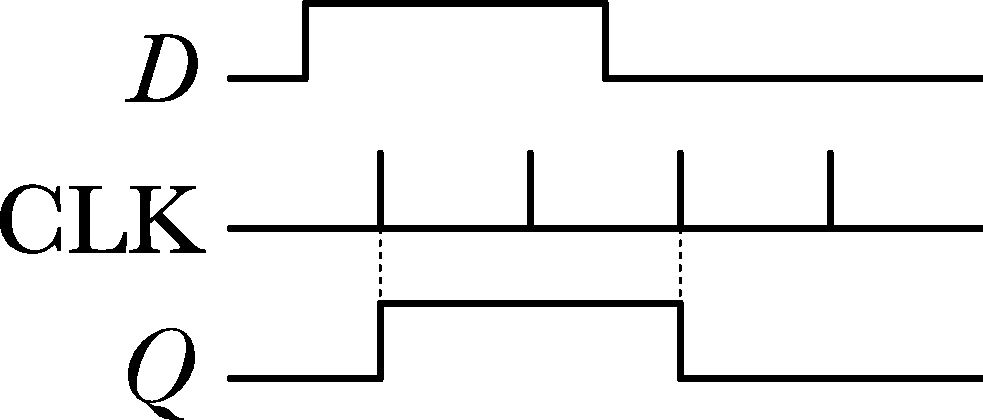
\includegraphics[width=5cm]{images/d_timing.pdf}
        \caption{D-FFのタイミングチャート}
      \end{minipage}
    \end{figure}
    \begin{table}[h]
      \begin{minipage}{0.49\hsize}
        \centering
        \caption{JK-FFの状態遷移表}
        \begin{tabular}{ccc||c}
          \hline
          $J$ & $K$ & CLK & $Q^+$ \\ \hline \hline
          $\times$ & $\times$ & 0 & $Q$ \\
          0 & 0 & 1 & $Q$ \\
          0 & 1 & 1 & 0 \\
          1 & 0 & 1 & 1 \\
          1 & 1 & 1 & $\overline{Q}$ \\ \hline
        \end{tabular}
      \end{minipage}
      \begin{minipage}{0.49\hsize}
        \centering
        \caption{D-FFの状態遷移表}
        \begin{tabular}{c||c}
          \hline
          CLK & $Q^+$ \\ \hline \hline
          0 & $Q$ \\
          1 & $D$ \\ \hline
        \end{tabular}
      \end{minipage}
    \end{table}

    JK-FFは, $J = K = 1$の時以外は$R = J$, $S = K$と見たときのRS-FFと同じ動作をする.
    $J = K = 1$の時は内部状態$Q$を反転させる.

    D-FFは, はCLKが0の時は現在の内部状態を保持し, それ以外は内部状態$Q$を$D$にする.
  \subsection{シフトレジスタの作成}
    簡単な順序回路の例として3ビットシフトレジスタを設計する.
    シフトレジスタは, クロック入力ごとに保持しているビット列を1桁ずつシフトさせる回路である.
    この操作の度に最上位ビットは捨てられ, 最下位ビットにはクロック入力時の入力が入る.
    構成方法としては, フリップフロップを直列に並べ, 下位ビットの内部状態を上位ビットに書き込むようにすればいい.

    D-FFを使用すれば簡単に構成することができるが, KENTAC 2600にはD-FFが2個しか内蔵されていないので,
    JK-FFを用いてD-FFと同じ動作をする回路を作成する.

    作成したD-FFを3つ直列に接続してシフトレジスタを作成する.
    このシフトレジスタの内部状態を$Q_3$, $Q_2$, $Q_1$とする.
    $Q_3$が最上位ビットである.
    また, 直近の入力$A$が$1 \rightarrow 1 \rightarrow 0$だった時に出力$X$が1になるようにする.
    これは, ($Q_3, Q_2, Q_1$)が(1, 1, 0)のときに$X$に1を出力すればいい.

    作成した回路を図\ref{fig:JK-FF_by_D-FF}, \ref{fig:shift_register}に示す.
    ただし, D-FFの入力, クロック入力をそれぞれ($D$, CLK), 出力を($Q$, $\overline{Q}$)とする.

    \begin{figure}[h]
      \centering
      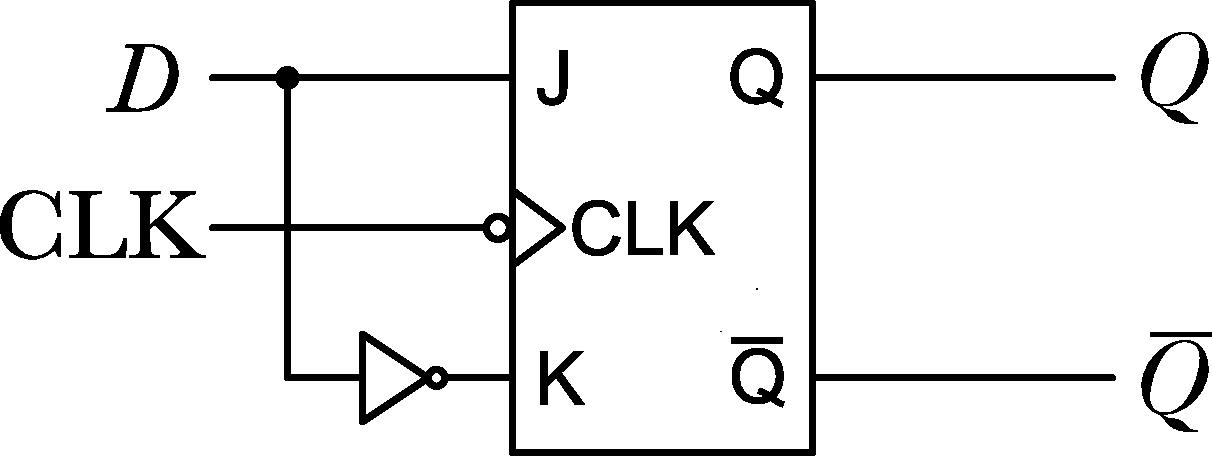
\includegraphics[width=8cm]{images/d_w_jk.pdf}
      \caption{JK-FFによるD-FF}
      \label{fig:JK-FF_by_D-FF}
    \end{figure}
    \begin{figure}[h]
      \centering
      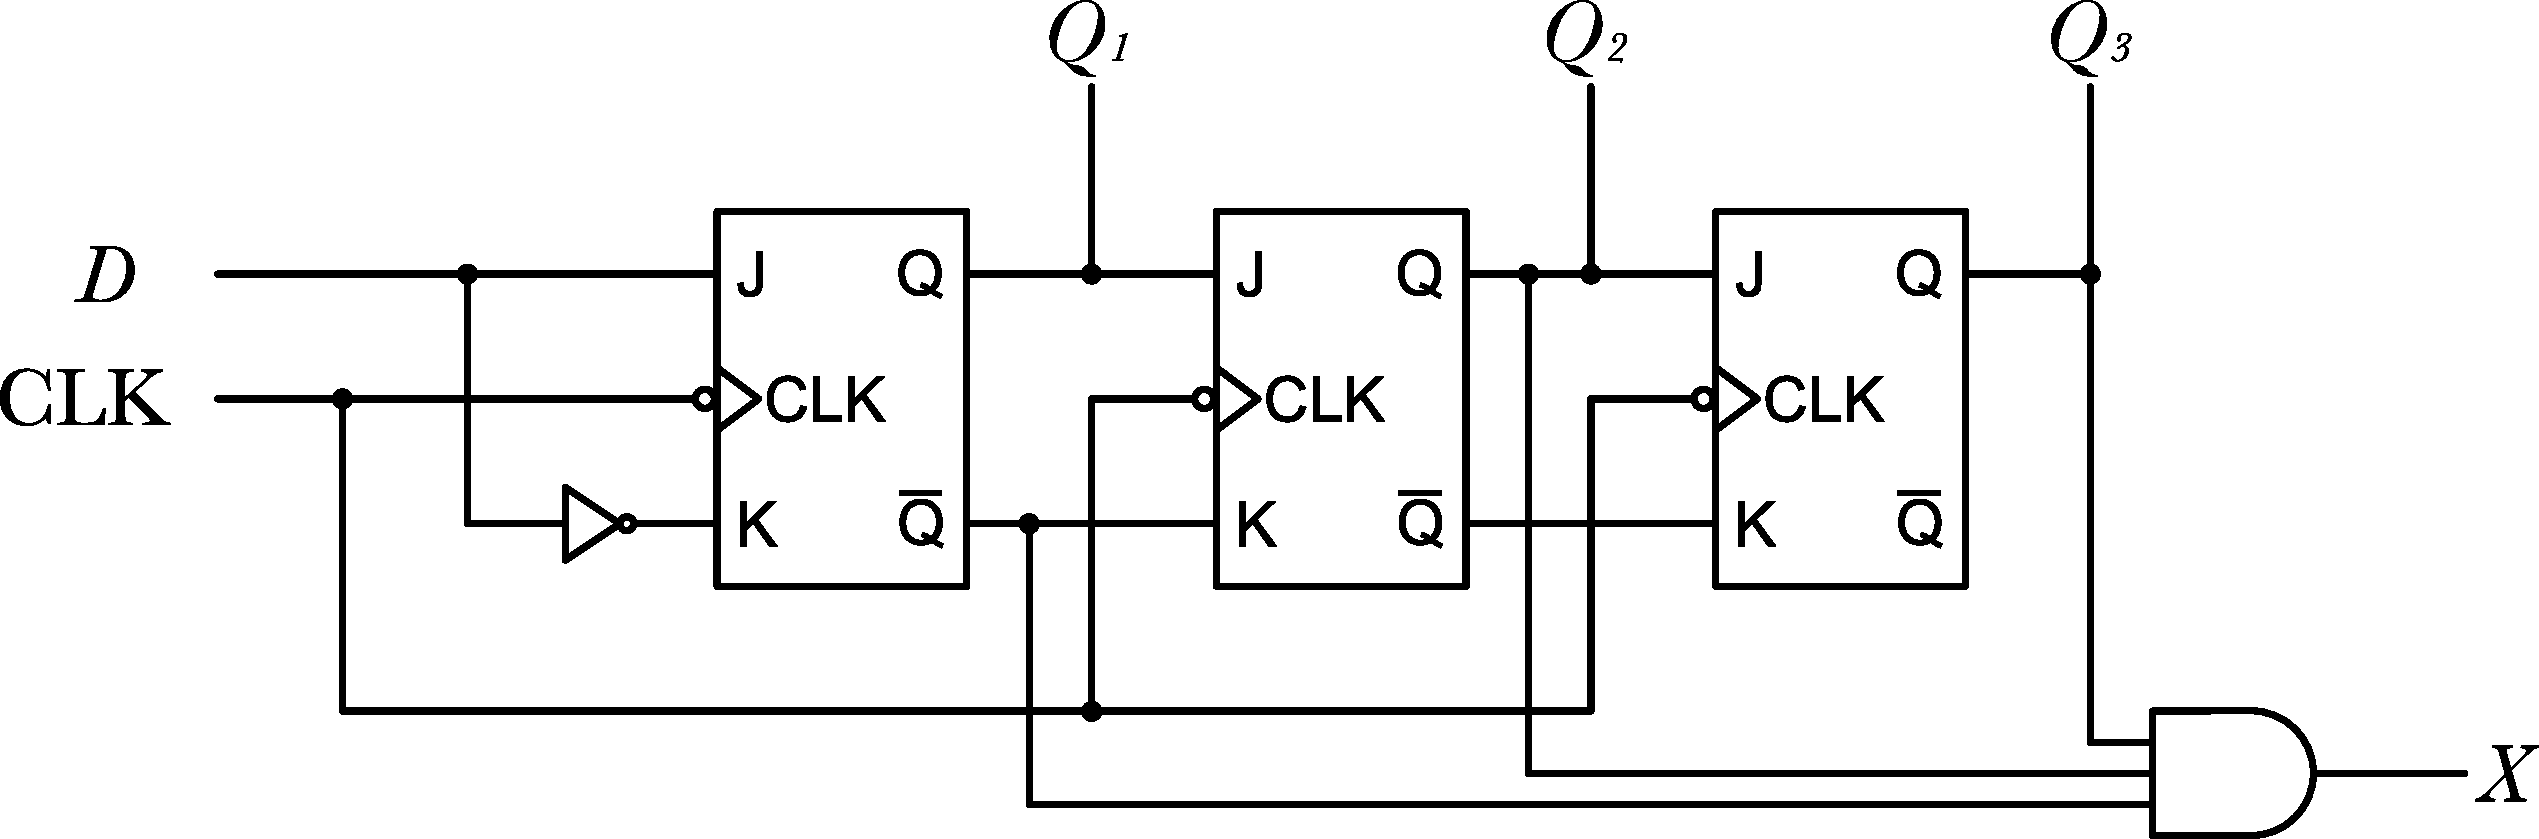
\includegraphics[width=15cm]{images/shift.pdf}
      \caption{3ビットシフトレジスタの論理回路}
      \label{fig:shift_register}
    \end{figure}
  \subsection{カウンタの作成}
    カウンタはクロック入力の回数を数える順序回路である.
    今回は3ビットの8進カウンタを設計する.
    始めに, 現在の内部状態を$(Q_3 \ Q_2 \ Q_1)_2$, 次の内部状態を$(Q_3^+ \ Q_2^+ \ Q_1^+)_2$として
    状態遷移表を表\ref{tab:counter}に示す.
    \begin{table}[h]
      \caption{8進カウンタの状態遷移表}
      \label{tab:counter}
      \centering
      \begin{tabular}{ccc||ccc}
        \hline
        $Q_3$ & $Q_2$ & $Q_1$ & $Q_3^+$ & $Q_2^+$ & $Q_1^+$ \\ \hline \hline
        0 & 0 & 0 & 0 & 0 & 1 \\
        0 & 0 & 1 & 0 & 1 & 0 \\
        0 & 1 & 0 & 0 & 1 & 1 \\
        0 & 1 & 1 & 1 & 0 & 0 \\
        1 & 0 & 0 & 1 & 0 & 1 \\
        1 & 0 & 1 & 1 & 1 & 0 \\
        1 & 1 & 0 & 1 & 1 & 1 \\
        1 & 1 & 1 & 0 & 0 & 0 \\ \hline
      \end{tabular}
    \end{table}

    次に, この表から$Q_3^+$, $Q_2^+$, $Q_1^+$の論理式を導く.
    各フリップフロップは, 自身より下位のビットが全て1になった時に反転すれば良いので,
    下位ビット全ての論理積を取り,
    JK-FFの両方の入力端子に入力\footnote{\ref{subsec:jk_and_d}より,
    $J$, $K$両方に1を入力をすると反転する}するように設計する.
    $Q_3$, $Q_2$, $Q_1$それぞれの入力を($J_3, K_3$), ($J_2, K_2$), ($J_1, K_1$)として
    求めた論理式をまとめると,
    \begin{eqnarray*}
      J_1 &=& K_1 = 1 \\
      J_2 &=& K_2 = Q_1 \\
      J_3 &=& K_3 = Q_1Q_2
    \end{eqnarray*}
    となる.

    この式をもとに作成した回路を図\ref{fig:counter}に示す.
    \begin{figure}[h]
      \centering
      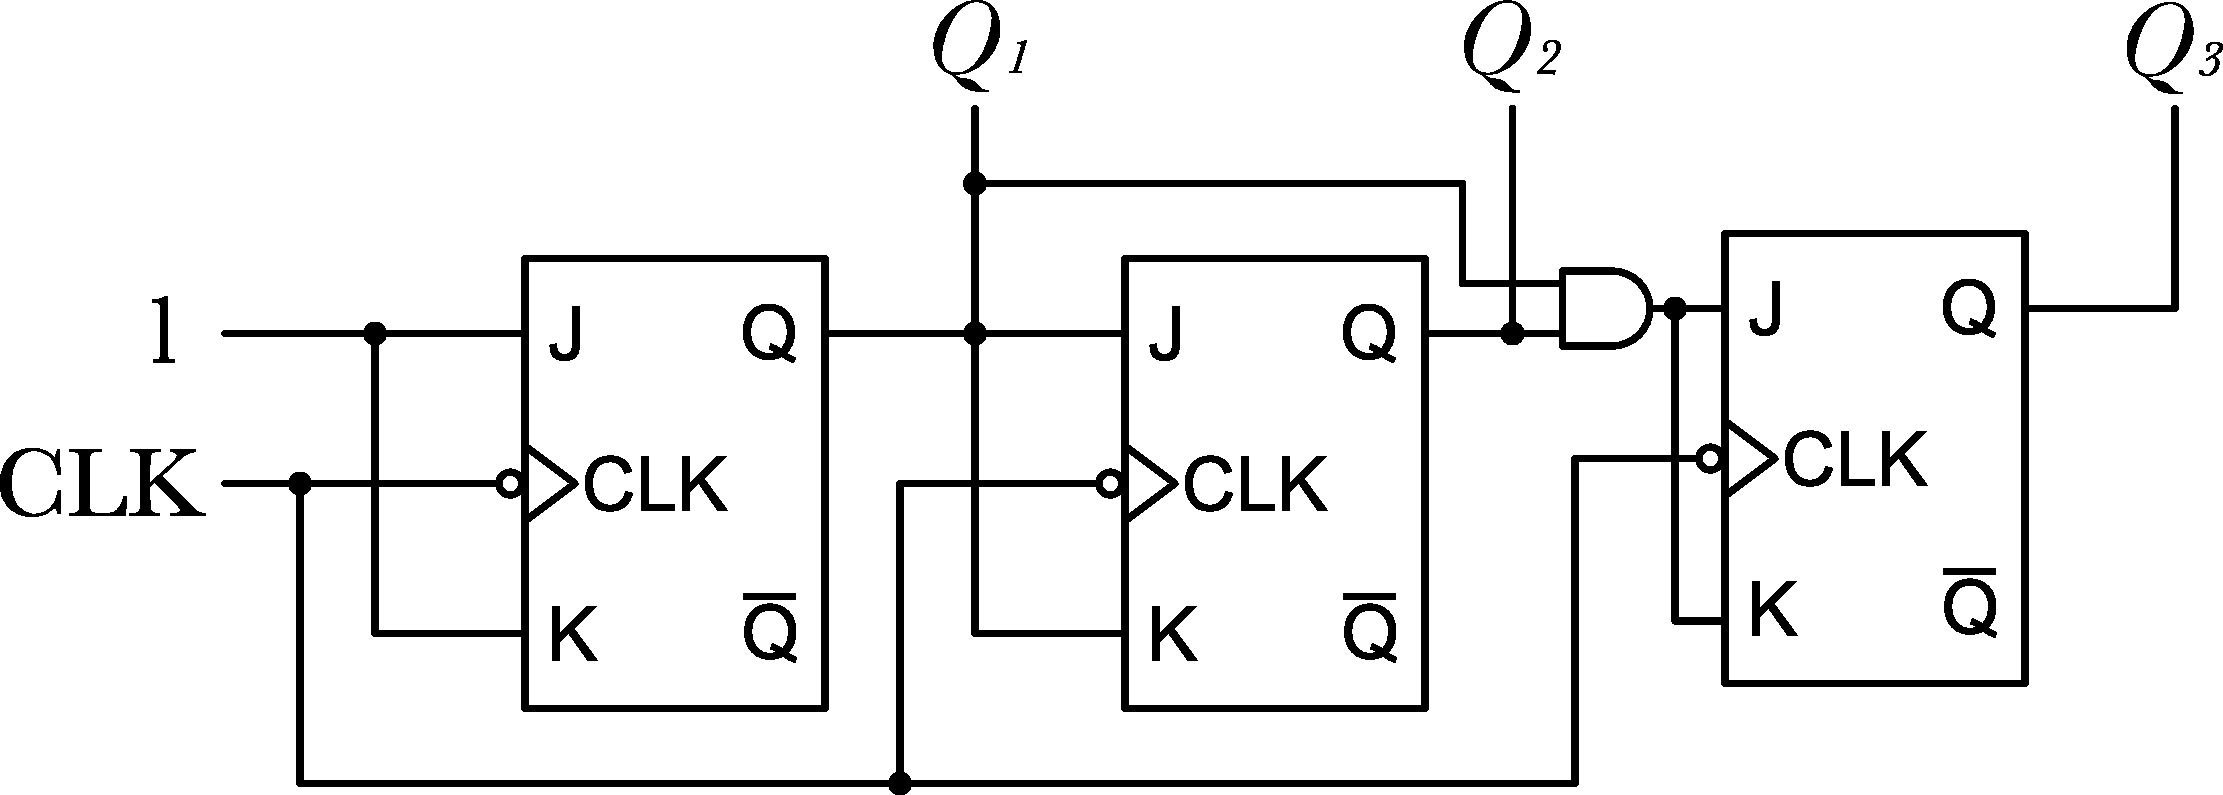
\includegraphics[width=13cm]{images/counter.pdf}
      \caption{8進カウンタの論理回路}
      \label{fig:counter}
    \end{figure}
\section{調査課題「SRAMについて」}
  SRAM(Static Random Access Memory)とは, コンピュータ内でCPUと主記憶の間にあるキャッシュメモリに使われている.
  RAMとは, 読み書き可能だがコンピュータの電源を切るとデータが消えてしまうメモリであるが,
  反対に書き込み不可能だが電源を切っていてもデータを保持できるROM(Read Only Memory)もある.

  また, SRAMと似た装置としてDRAM(Dynamic Random Access Memory)があり,
  これもSRAMと同様にキャッシュメモリに使用されている.

  特にSRAMは自然放電によるデータ損失がないので,
  コンピュータの高速処理を実現している.

  この2つのそれぞれの特徴を表\ref{tab:SRAM_and_DRAM}にまとめる.

  \begin{table}[h]
    \centering
    \caption{SRAMとDRAM}
    \label{tab:SRAM_and_DRAM}
    \begin{tabular}{c|cc}
      & SRAM & DRAM \\ \hline
      動作速度 & 速い & 遅い \\
      消費電力 & 小さい & 大きい \\
      容量 & 大きくしづらい & 大きくしやすい \\
      コスト & 高い & 安い \\
    \end{tabular}
  \end{table}

  この表からわかるように, 性能はSRAMの方が高い.
  さらに, 上の表に加えて, DRAMはSRAMに比べて定期的に電流を流さないとデータが消えてしまうので,
  処理に遅延が発生する.
  性能だけを見るとSRAMが高いが, コストも高いので
  キャッシュメモリの中でも特に重要な部分をSRAM, そうでない部分をDRAMと使い分けている.
\section{感想$\cdot$意見}
  今回の実験では, 動作をもとに回路を設計することを中心に行った.
  今までの授業などでは, 真理値表とカルノー図などから論理的に式を起こして回路を実装していたが,
  今回の実験を通して直感的に回路を組むことを覚えた.

  今回学んだ内容を次回以降の実験や, 今後の授業に生かしていきたい.
\section*{参考文献}
  \begin{enumerate}
    \item 令和元年度電子制御工学実験3年後期テキスト
    \item わわわIT用語辞典 SRAM, https://wa3.i-3-i.info/word17052.html, 2019/12/12
    \item ITポスト.com メモリとは、RAMとROMの違い,
      \\http://xn--l8jcc0l6q2czg5j.com/2017/10/31/post-1263/, 2019/12/12
  \end{enumerate}
\end{document}
